% !Mode:: "TeX:UTF-8" 

\BiChapter{绪论}
{Introduction}

\BiSection{课题背景及研究目的和意义}
{Background, Research Objective and Significance}

随着计算机软件广泛应用于经济、军事、商业等各个领域中,软件质量问题日益引起了人们的广泛重视。保证软件质量、提高软件可理解性和可维护性已经成为软件系统开发和维护工作的一个不可或缺的重要方面。随着应用需求和应用环境的不断变化,现实世界中的软件系统会随着时间而不断演化。在软件开发和维护的过程中,软件开发人员会向软件系统中不断添加新的功能,将导致软件规模越来越大、逻辑越来越复杂,致使软件的质量、可理解性和可维护性也会随着时间逐渐下降。

与此同时,代码复用作为一种常见的软件开发手段,尽管可以提高软件开发效率,但同时也会向软件系统中引入大量的克隆代码。有研究表明:软件工程实践中,软件开发人员通过复制和粘贴操作向系统中引入多种类型的克隆代码(Code Clone)\cite{roy2007survey}。克隆代码在大型软件系统中会占到代码总量的7\%-23\%\cite{baker1995finding,kontogiannis1996pattern,lague1997assessing},甚至在有的软件系统中占到59\%\cite{ducasse1999language}。大量的克隆代码使得软件变得越来越难以理解,降低了软件的可理解性。克隆代码会随着软件系统演化,在演化中可能会被软件开发人员修改而发生变化,从而降低软件可维护性。具体来说,由于克隆代码之间的相似性,对某一个克隆代码的修改可能会导致其它克隆代码的变化,将之称为克隆代码的一致性变化(Clone Consistent Change)。克隆代码的一致性变化问题不仅仅会导致软件系统额外的维护代价;遗忘克隆代码的一致性变化还会导致克隆代码的一致性违背缺陷(Clone Consistency-Defect),降低了软件的可维护性,从而进一步降低软件质量。因此,Fowler将克隆代码视为一种代码坏味(Bad Smell)\cite{fowler2009refactoring},认为克隆代码的存在会对软件系统造成不可避免的影响,例如对克隆代码相关缺陷的研究\cite{juergens2009code,gauthier2013uncovering,wagner2016relationship}、对克隆代码的有害性研究\cite{kapser2008cloning,selim2010studying,wang2012can}等。
因此,克隆代码是影响软件质量、可理解性和可维护性的一个重要因素,如何分析和理解系统中既有的克隆代码,并对其进行有效地维护是一个值得研究的问题。目前,对克隆代码的分析和维护研究已成为软件工程领域中的一个研究热点问题,同时也是亟待解决的一个问题。

为解决克隆代码问题,研究人员展开了大量且深入的研究,并取得了较多的研究成果。目前对克隆代码的研究包含三个主要的研究内容,即克隆检测研究、克隆分析研究和克隆维护研究。克隆检测研究是最早也是研究最为充分的一个研究内容,旨在从软件系统中检测已经存在的克隆代码。到目前为止,研究人员提出和开发了许多克隆代码检测的方法和工具,例如NiCad\cite{roy2008nicad}、CCFinder\cite{kamiya2002ccfinder}、Deckard\cite{jiang2007deckard}等等。但是,由于系统存在着大量的克隆代码并且情况复杂,目前克隆检测的效果并不能完全令人满意。更为重要的是,克隆检测研究既不能消除克隆代码,也不能消除克隆代码对软件产生的不利影响,因此无法直接帮助提高软件的质量及其可维护性。而对克隆代码的分析和维护研究可以弥补这一不足之处,本文通过对克隆代码的分析和维护研究,旨在帮助开发人员理解和维护软件系统中的克隆代码,并帮助提高软件质量、软件可理解性和可维护性。

克隆代码分析是目前克隆代码研究中较为活跃的一个研究内容,其主要目的是帮助软件开发人员理解系统中存在的克隆代码。研究发现克隆代码会随着软件演化而演化\cite{kim2005empirical,saha2011automatic},在其演化过程中克隆代码会对软件系统产生影响,同时也表现出了不同的特征\cite{gode2011frequency,mondal2012dispersion,rahman2014change}。如何深入的分析克隆代码及其演化情况,从而揭示克隆代码所隐含的信息是一个值得研究的问题。通过对克隆代码的演化分析,并获取克隆代码的演化特征,对于维护人员理解克隆代码及其演化过程具有积极的意义,可以提高软件的可理解性。

克隆维护研究是克隆研究的另一项重要内容,旨在帮助软件开发人员维护系统中的克隆代码、解决克隆代码可能引发或者已经所引发的问题。在克隆代码的演化过程中,克隆代码可能会被程序开发人员修改而发生变化 ,并可能引发克隆代码的一致性变化\cite{krinke2007study,aversano2007clones}。克隆代码的一致性变化会对软件系统产生较大的影响:首先,确认克隆代码是否需要一致性变化和执行克隆代码的一致性变化,会增加软件维护代价;其次,遗忘克隆代码的一致性变化会导致克隆代码的一致性违背缺陷的产生\cite{juergens2009code,wagner2016relationship},会进一步增加软件维护代价。因此,如何避免和预测克隆代码的是否需要一致性维护(Clone Consistency-Maintenance),是另一个值得研究的问题。通过预测克隆代码的一致性维护需求,不仅可以降低克隆所导致的维护代价,还可以有效地避免克隆代码的一致性违背缺陷,从而帮助提高软件质量和可维护性。

基于以上分析,本文研究基于软件演化的克隆代码分析与一致性维护方法,旨在帮助开发人员在软件开发过程中理解和维护软件系统中的克隆代码。首先,本文结合软件与克隆代码的演化过程,研究并提取克隆代码演化特征,揭示克隆代码及其演化过程所隐含的信息,为克隆代码的一致性维护需求预测研究奠定了基础。然后,针对克隆代码一致性变化导致的额外维护代价和一致性违背缺陷的问题,分别在克隆代码创建时和克隆代码变化时,预测克隆代码的一致性维护需求,帮助开发人员降低克隆代码的维护代价和避免相关的一致性违背缺陷。最后,结合软件开发过程,针对软件开发初期系统中缺少相应的数据的问题,研究跨项目的克隆代码一致性维护需求预测方法,使用不同系统的数据预测软件系统的克隆代码一致性维护需求。本文所提出的方法可在软件开发过程中帮助开发人员边开发、边维护克隆代码,帮助提高软件质量和软件的可理解性和可维护性。


\BiSection{国内外研究现状及其分析}
{Related Work}

在目前对克隆代码的研究中,尚没有统一的克隆代码的形式化定义。但研究人员普遍认为克隆代码是根在某种相似性定义的作用下彼此相似的代码片段\cite{roy2007survey}。按照克隆代码的语法和语义的相似度,研究人员将克隆代码划分为如下四种类型\cite{koschke2007survey}:
\begin{itemize}
\item 
Type-1克隆代码:除空格、格式和注释外,是完全相同的代码片段(简称1型克隆)。
\item 
Type-2克隆代码:除标识符、常量、类型外,是语法结构相同的代码片段(简称2型克隆)。
\item 
Type-3克隆代码:拷贝粘贴后修改的代码片段,如改变、增加或删除少量语句的代码,是语法结构相似的代码片段(简称3型克隆)。
\item 
Type-4克隆代码:执行相同的功能,但使用不同的语法结构实现的代码片段,是语义相似的代码(简称4型克隆)。
\end{itemize}

研究人员将Type-1的克隆代码称为精确克隆,表示完全相同的克隆代码。将Type-2和Type-3的克隆代码称为近似克隆,表示在语法相似的克隆代码。将Type-4的克隆代码称为语义相似的克隆代码。除此之外,也有研究人员研究其它类型的克隆代码,如函数克隆\cite{roy2008empirical}、模型克隆\cite{alalfi2012models}和结构克隆\cite{basit2009data,basit2005detecting}等。函数克隆指的是克隆代码为一个完整函数的克隆代码,函数克隆也可以按照语法语义分成Type 1-4克隆。同时,在模型驱动的软件开发过程中,会产生大量的模型文件。这类模型文件中相似的模型图(例如Simulink模型图)称为模型克隆。除此之外,有别于代码级别的克隆,结构克隆是较大粒度的克隆形式,一个结构克隆是一个包含若干个代码克隆的文件,可帮助软件开发人员分析文件和模块之间的关联程度。

\BiSubsection{研究热点与趋势}
{Research Hot-spots and Trends}

国内外对克隆代码的研究并没有软件工程的其它领域那么广泛,克隆代码研究仅仅是软件工程领域的一个较为细小的分支,克隆代码领域的文献数量也未达到较大的规模。
但是,克隆代码很早就引起了研究人员的注意,迄今为止研究人员对克隆代码的研究已有超过20年的时间。目前,克隆代码研究已经称为了软件工程领域的一个重要分支,每年均召开克隆代码研讨会(International Workshop on Software Clones),并与软件维护的相关会议一起举办,如SANER、WCRE等等。

为方便研究人员查阅相关研究,截止到2013年,阿拉巴马大学维护了一个克隆代码领域的文献库\footnote{  阿拉巴马大学关于克隆代码的文献库:http://students.cis.uab.edu/tairasr/clones/literature/。},并按照研究内容和目标将对克隆代码的研究划分为以下四个方向(如图~\ref{literaturedistribution1}~所示):

\begin{itemize}
\item
克隆检测方向:该方向目录下列出了与克隆代码检测相关的研究内容,旨在使用不同的方法从系统中检测出克隆代码。
\item 
克隆分析方向:该方向目录下列出了与克隆代码分析相关的研究内容,旨在帮助程序开发人员分析系统中存在的克隆代码,从而理解克隆代码。
\item 
克隆维护与管理方向:该方向目录下列出了与克隆代码维护与管理相关的研究内容,旨在通过各种技术手段维护和管理系统中的克隆代码。
\item 
综述和工具评估方向:该方向目录下列出了克隆代码综述和克隆检测工具评估相关的研究内容。
\end{itemize}

\begin{figure}[h]
\centering
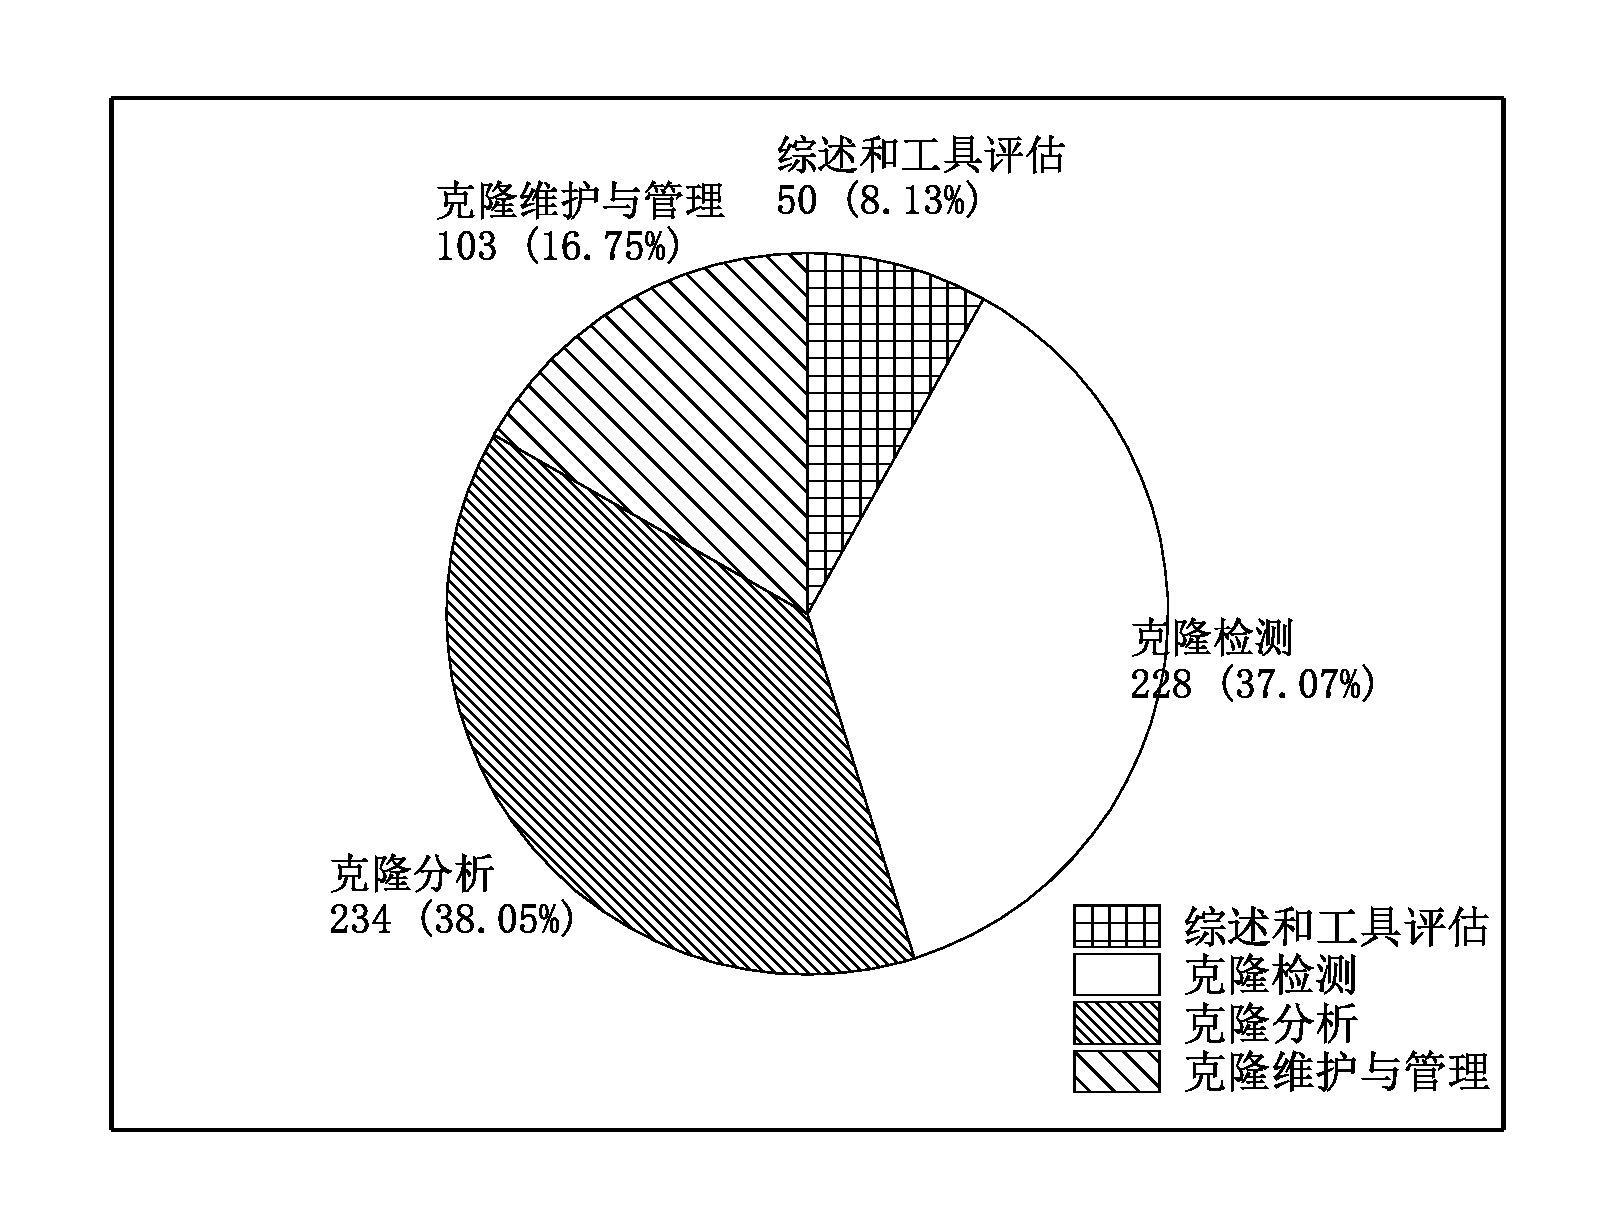
\includegraphics[width = 0.7\textwidth]{literaturedistribution1.pdf}
\bicaption[literaturedistribution1]{}{克隆代码研究领域文献分布情况}
{Fig.$\!$}{Literature distribution of code clone research}
\vspace{-1em}
\end{figure}

根据此文献库,Roy分析了此文献库中每个研究方向的论文分布和研究进展情况\cite{roy2014vision},但此文献库仅更新至2013年。为了进一步分析和反映克隆代码研究的研究热点和发展趋势,本文在该文献库的基础上,检索和收集了截止到2016年的克隆代码的研究论文。本文所统计和收集的文献共分为三类,即软件工程领域的重要国际会议论文、国际期刊论文以及相关学位论文。其中,重要国际会议论文为461篇,期刊论文120篇,学位论文34篇,共计615篇\footnote{在收集的过程中,仅选取领域内权威期刊、会议以及学位论文(期刊和会议选自CCF所推荐的学术刊物目录以及克隆代码研讨会)。} 。

同时,图~\ref{literaturedistribution1}~也给出了克隆代码研究领域的文献分布情况。从图中可以看出,目前研究中对克隆检测与分析的研究较为充分,是克隆研究领域的研究热点,分别占比37.07\%和38.05\%;而克隆维护与管理的研究论文占比较少(占16.75\%)。

为分析克隆代码研究领域的发展趋势,本文按照发表年份和研究方向进行了统计。统计分析结果如图~\ref{literaturedistribution2}~和~\ref{literaturedistribution3}~所示,其中图~\ref{literaturedistribution2}~是领域整体上每年发表文献数量的统计情况,图~\ref{literaturedistribution3}~是在不同研究方向上每年发表文献数量的统计情况。

从图~\ref{literaturedistribution2}和图~\ref{literaturedistribution3}~可以看出,克隆研究可以划分为两个阶段:1990-2003年和2004-2016年。在2003年以前,克隆代码研究领域的文献数量较少。而在2004年以后的近10年内,克隆代码研究领域的文献数量快速增长,并且保持在一个较高的水平上,展现出了蓬勃的发展趋势。在2003年以前,克隆代码研究主要集中在克隆检测方向。在2004年以后,各个研究方向的文献数量都有了快速增长,其中尤以克隆检测和分析方向的发展最为迅速。这说明克隆检测和分析是目前研究最为充分和最为活跃的研究方向。相比之下,克隆维护和管理仅在近几年才引起人们的关注,文献数量占比相对较少,但已呈现出逐年增长和后来者居上的趋势。这说明克隆维护和管理正在逐渐成为克隆代码研究领域的新热点。

\begin{figure}[h]
\centering
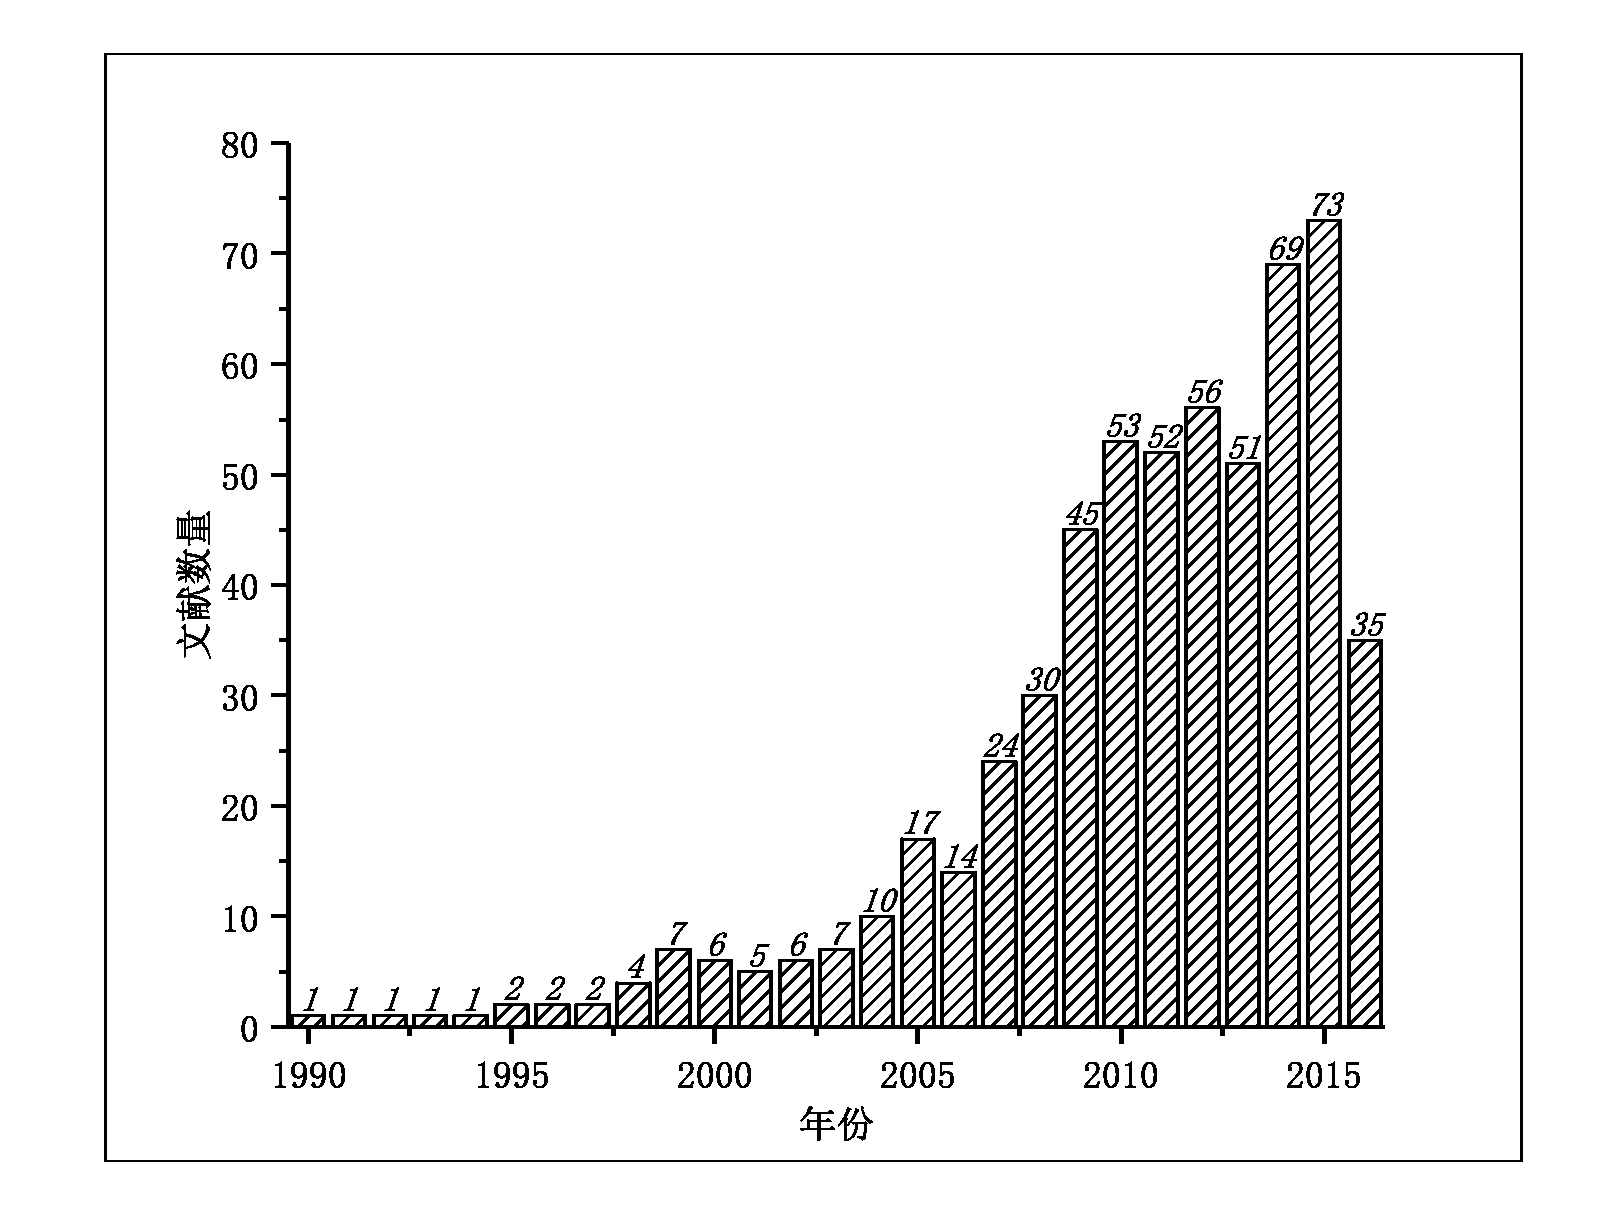
\includegraphics[width = 0.7\textwidth]{literaturedistribution2.pdf}
\bicaption[literaturedistribution2]{}{克隆领域每年发表的论文数量}
{Fig.$\!$}{Annual number of published papers of code clone research}
\vspace{-1em}
\end{figure}
\begin{figure}[h]
\centering
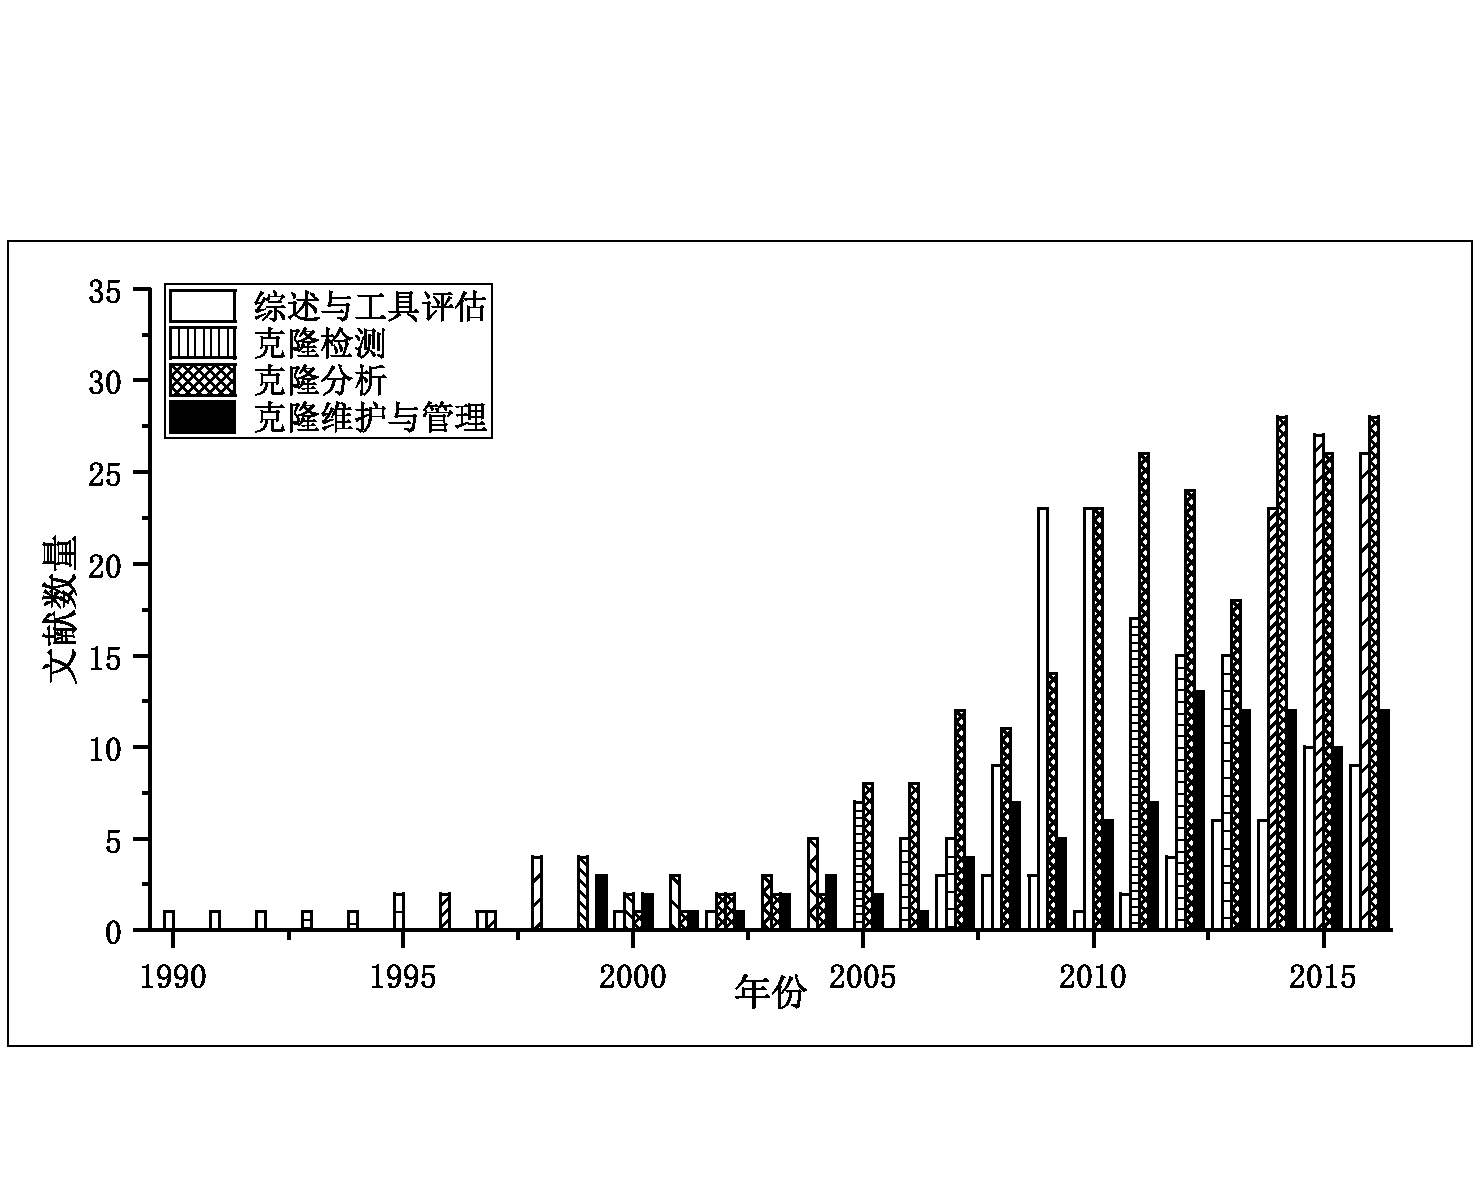
\includegraphics[width = 0.7\textwidth]{literaturedistribution3.pdf}
\bicaption[literaturedistribution3]{}{各个克隆研究活动每年发表的文献数量}
{Fig.$\!$}{Annual number of published papers of each clone research activity}
\vspace{-1em}
\end{figure}

\BiSubsection{克隆代码检测研究}
{Research on Code Clone Detection }
\label{ref-detection}

克隆检测是指从软件系统中检测克隆代码,并向软件开发人员报告克隆代码的活动。

一般而言,克隆代码检测过程分为三个步骤:代码的中间表示、相似性匹配和报告检测结果。“代码的中间表示”是使用不同的方法对源代码进行抽象表示或转换,将其表示为抽象语法树等一些中间表示形式。“相似性匹配”是对代码的中间表示形式进行相似性匹配与检测,寻找相似的代码片段。“报告检测结果”是将彼此相似的克隆代码以某种克隆组织方式存储检测结果,并向分析人员提供克隆检测报告。

\BiSubsubsection{克隆检测方法}
{Clone Detection Methods}

迄今为止,研究人员已提出了多种克隆检测方法,并同时也开发了相应的克隆检测工具。根据所使用的技术不同,可以将克隆检测划分基于文本(Text)、基于Token、基于树(如Abstract Syntax Tree,AST)、基于程序依赖图(Program Dependency Graph, PDG)和基于度量值(Metric)等方法。

基于Text的克隆检测方法是通过直接比较源代码文本,使用字符串匹配等算法来检测克隆代码。因其并没有对源程序进行词法分析,大部分仅可以较好地支持Type-1克隆代码的检测。目前,使用较多的基于文本的克隆检测工具主要有duploc\cite{ducasse1999language}、Simian\footnote{Simian - Similarity Analyser:http://www.harukizaemon.com/simian/index.html}%\cite{Simian}
、DuDe\cite{wettel2005archeology}、SDD\cite{lee2005sdd}、NiCad\cite{roy2008nicad}等。

基于Token的克隆检测方法是通过对源代码进行词法分析,获得源代码的Token序列,然后通过寻找Token序列中相似的子序列来检测克隆代码。因其对源代码进行了词法分析,所以可以较好地检测Type-2克隆代码的检测。但由于缺乏必要的语法和语义分析,使其无法较好地支持Type-3和Type-4克隆的检测。
目前,使用较多的基于Token的克隆检测工具主要有Dup\cite{baker1995finding}、CCFinder\cite{kamiya2002ccfinder}、CP-Miner\cite{li2006cp}、iClone\cite{gode2009incremental}、SourcererCC\cite{sajnani2016sourcerercc}等。

基于Tree的克隆检测方法是将源代码表示为某种树的形式(如抽象语法树、代码解析树等),然后通过使用子树匹配算法从中寻找相似的子树来检测克隆代码。因其对源代码进行了语法分析,所以提高了克隆代码检测的准确率,尤其是可以较好地支持Type-3克隆的检测。但是由于子树匹配算法的时间复杂度高于前两种方法,因此这类算法的检测速度低于前两种方法。
目前使用较多的基于Tree的克隆检测工具有CloneDr\cite{baxter1998clone}、SimScan\footnote{SimScan:http://www.blue-edge.bg/simscan/}%\cite{SimScan}
、Deckard\cite{jiang2007deckard}、CloneDigger\cite{bulychev2008duplicate}等。

前三种克隆检测方法中所使用的中间表示形式较为容易实现,可使用程序静态分析方法获得源代码的中间表示。事实上大部分的克隆检测方法和检测工具都属于前三种方法,并可以检测系统中的大部分的克隆代码。

基于PDG的克隆检测方法的主要思路是,将源代码转化成程序依赖图(包括数据依赖图和控制依赖图),然后通过寻找同构的子图来检测克隆代码。因程序依赖图表示了程序的语义信息,所以该方法可以支持语义相似的Type-4克隆代码的检测。但由于程序依赖图生成算法和图匹配算法的时间和空间复杂度极高,因而导致这类检测算法的时空开销过大,使其无法应用于大规模程序的克隆代码检测。
目前基于PDG的克隆检测工具主要有Duplix\cite{krinke2001identifying}等。

基于度量值的方法将源代码转换为某种中间表示,在其基础上提取度量值并抽象为一个特征向量,然后通过计算特征向量的相似度来检测克隆代码。该方法高度依赖于度量值的提取,在对源码提取度量值的过程中会损失源码的部分语义信息,因此检测效果不够理想,使其应用受限。

此外,还有人使用结合两种或两种以上检测技术的混合方法来检测克隆代码。例如,Deckard在生成抽象语法树的基础上提取结构特征向量表示代码,然后使用聚类的方法寻找克隆代码\cite{jiang2007deckard}。CloneMiner先将源代码表示为Token形式,然后在此基础上通过使用频繁模式挖掘算法寻找相似模式来检测克隆代码\cite{basit2009data}。White等人使用深度学习技术检测系统中的克隆代码\cite{white2016deep}。

\BiSubsubsection{克隆检测方法及工具评估}
{Evaluation for Code Clone Detection Methods and Tools}

不同的克隆检测方法和检测工具各有其优缺点,分别适合检测不同类型的克隆代码,对同一类型的克隆代码的检测效果也不尽相同。因此,通过对主流的克隆检测方法及其检测工具进行了评估\cite{bellon2007comparison,rattan2013software,roy2009comparison,svajlenko2014evaluating}。
Bellon对6个克隆检测工具进行了评估,分别对比了查准率、查全率以及时间和空间等性能\cite{bellon2007comparison}。Rattan通过使用一种标准的系统文献综述方法,详细分析了克隆检测方面的213篇文献,并对不同的检测方法进行了评估分析,并给出了未来的研究方向\cite{rattan2013software}。此外,Roy重点分析了检测工具的使用技术和适用环境,对克隆检测工具的检测效果进行了详细的对比,对帮助用户选择和使用克隆检测工具有重要的指导意义\cite{roy2009comparison}\cite{svajlenko2014evaluating}。

本文对目前较为主流的克隆检测工具和方法支持的克隆类型和检测效果等进行了评估,评估结果如表~\ref{detectionevaluation}~所示。其中,检测效果采用“较好”、“一般”和“较差”三种级别来评估\cite{rattan2013software}:“较好”是指可以较好地支持该类型克隆代码;“一般”是指可以支持检测该类型克隆代码,但效果不佳;“较差”是指可以检测少部分的该类型克隆代码;对未支持的克隆类型没有列出。

\begin{table}[h]
\bicaption[detectionevaluation]{}{主流克隆检测方法与工具评估}
{Table$\!$}{Evaluation for popular clone detection methods and tools}
\vspace{0.5em}
\centering
\wuhao
\begin{tabular}{cccc}
\toprule[1.5pt]
类型&工具或方法名&支持的克隆类型&检测效果\\
\midrule[1pt]
\multirow{5}{*}{Text} 
& Duploc\cite{ducasse1999language}&1、3&较好1,一般3\\
&Simian&1、2	&较好1,一般2\\
&DuDe\cite{wettel2005archeology}&1、3	&较好1,一般3\\
&SDD\cite{lee2005sdd}&1、3	&较好1,一般3\\
&NiCad\cite{roy2008nicad}&	1、2、3	&较好1、2、3\\
\hline
\multirow{4}{*}{Token} 
&Dup\cite{baker1995finding}&	1、2&较好1、2\\
&CCFinder\cite{kamiya2002ccfinder}&1、2&较好1、2\\
&CP-Miner\cite{li2006cp}&1、2、3&较好1、2,一般3\\
&iClone\cite{gode2009incremental}&1、2	&较好1,2\\
\hline
\multirow{4}{*}{Tree} 
&CloneDr\cite{baxter1998clone}&	1、2、3	&较好1、3,一般2\\
&SimScan&	1、2	&较好1、2\\
&Deckard\cite{jiang2007deckard}&	1、2、3	&较好1、2,一般3\\
&CloneDigger\cite{bulychev2008duplicate}&	1、2、3	&较好1、3,一般2\\
\hline
\multirow{2}{*}{PDG} 
&Duplix\cite{krinke2001identifying}&	1、2、3、4	&较好1、2,一般3,较差4\\
&Gabel\cite{gabel2008scalable}&1、2、3、4	&较好1、2、3,一般4\\
\hline
\multirow{2}{*}{Metric} 
&Kontogiannis\cite{kontogiannis1996pattern}&	1、2、3、4	&较好1、2,较差3、4\\
&Mayrand\cite{mayrand1996experiment}&	1、2、3、4	&较好1、2,较差3、4\\
\bottomrule[1.5pt]
\end{tabular}
\end{table}

从表~\ref{detectionevaluation}~可以看出,基于Text的检测工具不支持Type-4克隆的检测。对Type-1克隆的检测效果最好,对Type-3克隆的检测效果一般。而对Type-2克隆支持较弱,仅有两个工具可以支持。原因是Type-2克隆是标识符重命名的克隆代码,基于Text的方法不能很好地处理标识符重命名问题。
基于Token的检测工具同样不支持Type-4克隆的检测,但是可以较好地检测Type-1和Type-2克隆。支持Type-2克隆检测的原因是在将源程序转换成Token序列时进行了词法分析,因此可以解决标识符重命名的问题。
基于Tree的检测工具,同样不支持Type-4克隆的检测,但是对Type-1克隆的检测效果较好,并且几乎都支持Type-2和Type-3克隆的检测。由于采用的匹配算法不同,对Type-3即近似克隆的检测效果不尽相同,有些可以较好地支持Type-2克隆的检测,有些则较好地支持Type-3克隆的检测。
基于PDG的检测方法不仅可以较好地检测Type-1和Type-2克隆,还可以以不同的程度支持Type-3和Type-4克隆的检测。但因其复杂度相对较高,使其并没有太多的检测工具可以利用。
基于度量值的检测方法目前仅有一些检测方法被提出\cite{kontogiannis1996pattern,mayrand1996experiment},缺少相应的检测工具。

\BiSubsection{克隆代码分析研究}
{ Research on Code Clone Analysis}

克隆分析是指使用各种技术手段分析系统中的克隆代码,旨在帮助软件开发人员更好地理解和维护克隆代码。克隆分析研究主要包括克隆表示、克隆演化、克隆评价和克隆可视化等。

\BiSubsubsection{克隆代码表示}
{Code Clone Representation}

目前的很多克隆检测工具,如NiCad、CCFinder、iClone和Decard等,都使用检测报告的形式提供克隆代码的检测结果。由于不同的检测工具采用不同的技术检测克隆代码,因此不同的检测工具的克隆检测结果往往是不同的。

为了实现各个检测工具的克隆检测结果的共享,克隆检测工具iClone使用Rich Clone Format(RCF)表示克隆代码\cite{harder2011efficiently}。RCF不仅可以表示克隆代码的基本位置信息,还允许用户对其进行扩展,表示克隆代码的扩展信息。RCF 还定义了多种函数接口,以方便用户和其它检测工具检索克隆代码\footnote{RCF格式文档:http://www.softwareclones.org/rcf.php。}。但是,RCF并没有指出可以表示哪些具体的扩展信息以及以何种形式来表示这些信息。为表示克隆代码的上下文信息,Duala-Ekoko出了另一种克隆表示形式Clone Region Description(CRD)\cite{duala2010clone}。CRD采用一种与位置无关的克隆表示方法,CRD不保存克隆代码的位置信息,仅使用克隆代码本身及其所在文件的的语法信息、结构信息等表示克隆代码,有助于辅助开发人员跟踪克隆代码。

各种检测工具的克隆检测结果缺乏统一的表示形式,Harder在文献\cite{harder2013limits}中分析了统一克隆表示的挑战和限制,并给出了一个克隆表示的概念模型。Kapser也认为需要对克隆代码进行统一的表示,并提出了Unified Clone Model(UCM)模型\cite{kapser2012common}。UCM不仅可以表示克隆代码的基本位置信息,还可以表示克隆代码的上下文信息、演化信息和度量值信息等,具有较强的理论和实际意义\footnote{ UCM格式文档:http://www.softwareclones.org/ucm/index.php/Main\_Page。}。

\BiSubsubsection{克隆代码演化}
{Code Clone Evolution}
\label{ref-evolution}

克隆代码往往存在于软件系统的多个版本中,并随着软件系统进行演化。
克隆代码演化分析就是通过分析克隆代码的演化过程,识别克隆代码的演化规律,从而辅助人们更好地理解和维护克隆代码。

克隆代码存在于软件系统的多个版本中,并随着软件系统进行演化。克隆代码演化分析就是通过分析克隆代码的演化过程,提取克隆代码的演化特征,从而识别克隆代码的演化规律,辅助人们更好地理解和维护克隆代码。克隆演化研究包括克隆演化过程分析和演化特征分析两个方面。克隆演化过程分析即模型化克隆代码的演化过程。克隆演化特征分析是分析克隆代码在演化过程中表现出来的演化特征或演化模式及其对软件质量的影响。

克隆演化过程分析最早是2001年由Antoniol等人提出的,使用时间序列描述克隆代码的演化模型\cite{antoniol2001modeling}。2005年,Kim提出了克隆家系模型用于描述克隆代码的演化过程,是迄今为止最好的演化模型\cite{kim2005empirical}。而Roy使用函数映射帮助构建克隆家系,并开发了gCad克隆家系提取器,提升了构建克隆家系的效率\cite{saha2011automatic}。Bakota通过映射不同版本的克隆来分析克隆代码的演化过程,并使用克隆坏味(Clone Smell)帮助分析克隆代码对系统的影响\cite{bakota2011tracking}。Harder对现有的演化模型进行分析\cite{harder2009modeling},指出通过分析克隆演化特征可以帮助程序开发和维护人员理解和维护克隆代码。

目前,引发人们关注的演化规律主要包括:克隆寿命、克隆稳定性与一致性变化等研究。克隆寿命是指克隆代码在系统中的存在时间
克隆稳定性关注的是在克隆代码的生存期发生变化的问题。特别地,克隆代码的一致性变化往往会引发人们的强烈关注,原因在于克隆一致性变化可能会引发相关的软件缺陷,如标识符重命名缺陷等。

表~\ref{characteristic}~列出了目前对克隆演化特征的研究情况。由表~\ref{characteristic}~中可以看出,研究者较为关注的克隆演化特征是克隆寿命、克隆稳定性与一致性变化。上述三个特征并不是相互独立的,克隆寿命会受到稳定性和克隆变化的影响,同时克隆稳定性与克隆变化之间存在对立关系。对克隆演化分析的研究大多属于实证研究,往往会较多地依赖于具体被用于实验分析的软件系统,这就导致了不同的研究可能得出不同的结论。例如对克隆稳定性的研究就出现了截然相反的观点。尽管如此,克隆演化特征分析依然可以给开发人员提供有价值的建议。


\begin{table}[h]
\centering
\bicaption[characteristic]{}{克隆演化特征分析}
{Table$\!$}{The analysis of clone evolutionary characteristic}
\vspace{0.5em}
\wuhao
\begin{tabularx}{0.9\textwidth}{llX}
\toprule[1.5pt]
文献&克隆模式、特征&结论\\
\midrule[1pt]
\cite{kim2005empirical}&	克隆寿命/一致性变化	&观察并分析克隆家系寿命与一致性变化规律\\
\cite{cai2011empirical}&	克隆寿命&	克隆寿命与克隆修改次数、新增和减少有关\\
\cite{krinke2011cloned}&	克隆寿命&	克隆代码的寿命比非克隆的寿命更长\\
\cite{bazrafshan2012evolution}\cite{gode2009evolution}&	克隆比率/寿命/变化规律	&克隆比率会随时间降低,会存在超过一年,存在期间变化规律往往和具体系统相关\\
\hline
\cite{krinke2008cloned}&克隆稳定性&	克隆代码比非克隆代码更稳定\\
\cite{gode2011clone}\cite{harder2013cloned}&	克隆稳定性&	克隆代码十分的稳定\\
\cite{gode2011frequency}&	克隆变化/一致性变化&	大部分克隆不会变化,一致性变化会更少\\
\cite{rahman2014change}&	克隆稳定性&	克隆会比非克隆更容易发生变化\\
\cite{mondal2012comparative}\cite{mondal2012dispersion}&	克隆稳定性/变化分布&	Type-1、Type-2是不稳定的,Type-3是稳定的;发现克隆代码变化比非克隆更加分散,同时Type-3克隆比Type-1和Type-2更加分散\\
\hline
\cite{krinke2007study}&	一致性变化&	在发生变化的克隆代码中,约一半是一致性变化\\
\cite{barbour2011late}\cite{mondal2016comparative}&	延后传播&	Type-3更容易发生延后传播并导致缺陷\\
\bottomrule[1.5pt]
\end{tabularx}
\end{table}

\BiSubsubsection{克隆代码评价}
{Code Clone Evaluation}

克隆评价分析主要是分析克隆代码对系统产生的影响,以便辅助开发人员更好地维护克隆代码,克隆评价主要包括克隆相关的缺陷分析、克隆维护代价分析、克隆有害性分析等。

在早期,研究人员认为克隆代码是一种最刺鼻的代码坏味,是因为它有可能会引发相关缺陷。Juergens等人研究发现遗忘克隆代码的一致性变化容易引发相应的软件缺陷,从而降低了软件质量\cite{juergens2009code,inoue2012experience}。Gauthier在开源软件Joomla和Moodle中发现了几个潜在的影响软件质量的安全漏洞和缺陷\cite{gauthier2013uncovering}。但也有一些证据表明克隆代码并不一定会引发缺陷。例如,Bettenburg研究发现仅有极少数的不一致性变化会引发缺陷\cite{bettenburg2009empirical}。文献\cite{wagner2016relationship}的研究则表明Type-3克隆代码中大约有17\%的代码含有缺陷,且Type-3克隆不容易发生不一致性变化。文献\cite{elish2015fault}发现面向对象程序中的克隆类含有更少的缺陷,并且Type-3克隆含有的缺陷最少。因此,没有直接证据证明克隆代码与缺陷密切相关\cite{lo2012active,kamei2011empirical}。

研究人员还从维护代价的角度去分析克隆代码对软件产生的影响\cite{bakota2007clone}。Harder发现克隆代码并不会增加缺陷修复的时间,但未被修复缺陷会导致维护代价的增加\cite{harder2012controlled}。Lozano研究克隆代码的可变性发现克隆代码会增加软件维护的代价\cite{lozano2008assessing}。Juergens不仅认为克隆代码会增加维护代价,还提出了一个模型计算克隆维护代价\cite{juergens2010much}。Monden发现尽管克隆代码与软件可靠性和维护代价有一定的关联,但这种关联关系并不十分明确\cite{monden2002software}。

近些年来,研究人员也展开了克隆代码有害性分析的研究。Kapser发现在Apache中大约有71\%的克隆代码是有益的,且Apache Web Server中的克隆代码增加了系统的功能性,对软件维护具有积极的影响\cite{kapser2006cloning,kapser2008cloning,kapser2006supporting}。Selim发现克隆代码并不比非克隆代码具有更高的风险\cite{selim2010studying}。Wang提出利用贝叶斯网络对克隆代码进行有害性预测的方法\cite{wang2012can}。Higo对克隆代码进行过滤、合并等操作来提取有问题的克隆代码,在Linux内核2.6.6上的实验结果表明只有少数克隆代码是有问题的克隆代码\cite{higo2009problematic}。Hordijk提出的一个结构化的证据模型发现只有少部分的证据证明克隆代码是有害的\cite{hordijk2009harmfulness}。

表~\ref{evaluation}~对克隆评价分析研究进行了分类统计,使用“积极”、“中立”和“消极”三种评价标准对现有的克隆评价分析方法进行了总结。“积极”是指克隆代码的存在对系统有积极的影响;“中立”是指克隆代码不会对系统产生影响;“消极”是指克隆代码会对系统产生消极的影响。从表中可以看出,大部分研究对克隆代码持积极和中立的态度,仅有少数持消极态度。

\begin{table}[htbp]
\centering
\bicaption[evaluation]{}{克隆评价分析}{Table$\!$}{The analysis of clone evaluation}\vspace{0.5em}\wuhao
\begin{tabularx}{0.9\textwidth}{lllX}
\toprule[1.5pt]
&文献&评价&结论\\
\midrule[1pt]
\multirow{6}{*}{{克隆缺陷}} 
&\cite{juergens2009code}&消极&研究发现克隆代码的变化在克隆中发生较为频繁,同时也会导致相应的缺陷\\
&\cite{gauthier2013uncovering}&消极&通过对不安全的克隆代码分析,发现了几个安全漏洞和缺陷\\
&\cite{bettenburg2009empirical}&积极&克隆代码的变化并不会引入相关缺陷,不会对软件的质量产生影响\\
&\cite{elish2015fault}&积极&克隆代码含有更少的缺陷,Type-3所含有的缺陷最少\\
&\cite{lo2012active}&中立&克隆代码研究应用到缺陷检测中,但没有直接证据证明与缺陷相关\\
&\cite{kamei2011empirical}&中立	&通过实验发现并不会增加缺陷修复时间,但是缺陷未被修复,可能会产生维护代价的增加\\
\midrule[1pt]
\multirow{4}{*}{{维护代价}} 
&\cite{wagner2016relationship}&中立	&Type-3克隆中有17\%含有缺陷,并且Type-3克隆更容易发生一致性变化\\
&\cite{harder2012controlled}&消极&通过对克隆代码的可变性研究发现克隆代码确实会增加其方法可变化的维护代价,但没有确切的证明会说明克隆会增加系统维护代价\\
&\cite{juergens2010much}&消极&认为克隆会增加维护代价,并且提出了一个代价计算模型计算这次代价\\
&\cite{monden2002software}&中立&Monden却发现包含克隆的模块比不含克隆的模块更可靠,同时含有大量克隆的模块却相反实验表明了克隆与系统可靠性和维护代价的关系,但是这种关系仍然不够明朗\\
\midrule[1pt]
\multirow{6}{*}{{克隆有害性}} 
&\cite{selim2010studying}&积极&克隆代码并不比非克隆代码具有更高的有害风险\\
&\cite{kapser2006cloning}\cite{kapser2008cloning}&积极	&发现最多有71\%的克隆对系统的可维护性具有积极的影响\\
&\cite{rahman2012clones}&积极	&克隆并不是真正的代码坏味,克隆是无害的\\
&\cite{wang2012can}&中立	&预测克隆有害性,其中有害的较少,无害的较多\\
&\cite{higo2009problematic}&中立&使用分类模型抽取有问题的克隆代码,只有少部分是有问题的克隆\\
&\cite{hordijk2009harmfulness}&中立&现有研究不能支撑克隆有害的观点,仍需进一步的研究\\
\bottomrule[1.5pt]
\end{tabularx}
\end{table}

\BiSubsubsection{克隆代码可视化}
{Code Clone Visualization}

克隆检测工具通常使用文本形式来保存克隆代码的检测结果。但是,用文本形式保存大量的检测结果,既不形象直观,也不利于深入分析克隆代码的分布情况和关联关系。因此,展开了对克隆代码进行了可视化研究。克隆可视化是使用可视化技术将克隆代码在软件中的分布情况以及克隆关系以图形的方式展现出来,以辅助开发人员更加方便直观地理解、分析和维护克隆代码。

目前,使用较多的可视化技术主要有捆绑图、散点图和树图。捆绑图是从宏观的角度展示克隆文件之间的关系以及克隆关系的强弱。一般以克隆文件为粒度,采用同心圆环、扇形和曲线相结合的形式可视化克隆代码\cite{hanjalic2013clonevol,hauptmann2012using,voinea2014visual}。例如可视化工具ClonEvol使用分层捆绑图分析软件的演化情况,以辅助开发人员寻找自己感兴趣的克隆代码\cite{hanjalic2013clonevol}。Hauptmann则使用捆绑图分析软件各模块之间的耦合关系\cite{hauptmann2012using}。
散点图是从微观的角度使用矩阵的形式对软件中克隆代码的分布情况进行可视化\cite{cordy2011exploring,higo2007method,livieri2007very}。Cordy使用散点图分析软件之间的相似性\cite{cordy2011exploring},Higo则使用散点图分析软件中的克隆模式\cite{higo2007method,livieri2007very}。
树图是以二维矩形图的形式对克隆代码在软件中的分布情况和层次结构进行可视化,以树图形式可视化克隆代码的工具有VisCad\cite{asaduzzaman2011viscad,uddin2015comprehension}、SoftGUESS\cite{adar2007softguess}。

克隆可视化的作用不仅仅是可视化克隆代码,更重要的作用是通过克隆代码的可视化辅助软件开发人员分析克隆代码对软件产生的影响。例如可视化工具Doppel-Code可以用于分析克隆代码对系统全局和局部产生的影响,并将不同克隆代码组对系统的影响进行排序\cite{forbes2012doppel}。Jiang提出一个克隆可视化框架,辅助开发人员分析系统内各模块间的耦合和内聚情况\cite{jiang2007framework,jiang2006visualizing}。Zhang等人通过对结构克隆进行过滤和可视化分析,帮助维护人员寻找对开发人员有用的克隆代码以便进行代码复用\cite{zhang2008query}。

\BiSubsection{克隆代码维护研究}
{Research on Code Clone Maintenance}

克隆维护是解决克隆代码问题的直接途径,主动地解决克隆代码可能或已经引发的问题。克隆代码维护与软件开发过程结合得较为紧密,目前的研究主要包括克隆重构、克隆复用、克隆规避和克隆管理方法。

\BiSubsubsection{克隆代码重构}
{Code Clone Refactoring}
\label{ref-clonerefactoring}

重构作为一种常见的软件维护手段,是指在不改变软件外部行为的条件下改变软件的既有设计\cite{kerievsky2006重构与模式}。将重构应用于克隆维护中,指的是通过重构手段消除系统中的克隆代码。克隆代码的重构研究是对克隆代码维护研究的一个主要的研究内容。

由于重构所需的条件较为苛刻,在重构前对克隆代码进行可重构性分析和重构排序显得尤为重要。可重构性分析旨在识别适于重构的克隆代码候选集合,以提高克隆重构的效率\cite{lin2014detecting,mende2009evaluation,schulze2008towards,choi2011extracting}。Lin等人通过对克隆代码进行差异性分析帮助开发人员决定是否进行重构操作和如何执行重构操作\cite{lin2014detecting}。Mende实现了一个工具在软件中识别可以被重构的函数克隆\cite{mende2009evaluation}。Schulze通过计算克隆代码的可重构指数识别可重构的克隆代码\cite{schulze2008towards}。Choi等人提出了基于度量值的可重构性分析方法,可以快速地识别可重构的克隆代码\cite{choi2011extracting}。

识别可重构克隆后,为了节省重构时间,还可以对克隆代码进行重构排序或者调度\cite{mandal2014automatic,lee2011automated,zibran2011constraint}。Mandal先通过分析克隆演化模式来确定克隆候选,然后使用关联规则挖掘进行可重构排序\cite{mandal2014automatic}。Lee采用遗传算法对重构进行调度,以确定重构顺序帮助改进软件质量\cite{lee2011automated}。Zibran提出一种极限编程方法对克隆代码进行重构调度\cite{zibran2011constraint}。Liu等人提出了一个重构调度方法帮助优化调度过程\cite{liu2012schedule}。Radhika等人从重构代价的角度对所有的克隆代码进行重构排序\cite{venkatasubramanyam2013prioritizing}。Tsantalis也对克隆代码的可重构性进行了分析,并获得一些有用的结论\cite{tsantalis2015assessing}。

克隆重构最主要的目的是消除系统中的克隆代码,研究人员提出了许多具体的重构方法\cite{higo2008metric,krishnan2014unification,barbosa2013removing,ettinger2017efficient}。Higo等人开发了一个工具ARIES,通过计算不同的度量值来确定使用哪一种目前已有的重构方法移除克隆代码\cite{higo2008metric}。Krishnan分析克隆代码的程序依赖图,并通过检测和参数化克隆代码的差异点对克隆代码进行重构\cite{krishnan2014unification}。Barbosa使用四种规则重构克隆代码,实验结果表明基于规则的重构方法可以有效地移除软件中的克隆代码\cite{barbosa2013removing}。Ettinger等人提出了一个高效的方法可以消除系统中的Type-3克隆代码\cite{ettinger2017efficient}。

在重构完成后,对重构后代码进行分析,还可以得出一些结论以进一步指导克隆重构\cite{gode2010clone,zibran2013evaluating,eunjong2014investigation,eunjong2014investigation}。G{\"o}de研究发现在不同的软件系统中都存在克隆重构的行为,并且克隆重构不是经常性地发生而是有选择性地发生\cite{gode2010clone}。Zibran等人研究发现克隆规模对克隆重构没有重要的影响,同时在软件早期的版本中重构会较为频繁地发生,发生重构的克隆在重构前往往是较为稳定的克隆代码\cite{zibran2013evaluating}。Choi识别出几种较为频繁的克隆重构模式,并且分析了每种重构模式的特征\cite{eunjong2014investigation}。Tairas提出了子克隆的概念,并发现子克隆的重构行为更容易发生\cite{tairas2010sub}。

\BiSubsubsection{克隆代码复用}
{Code Clone Reuse}

近些年来,随着对克隆代码评价分析研究的深入,人们已经意识到复用健壮性好的克隆代码不仅有助于缩短软件开发周期,还有利于提高软件的健壮性和可维护性。

Krutz等人提出克隆数据库概念,将已有克隆代码组织为克隆数据库,并结合代码检索技术实现对克隆代码的复用\cite{krutz2014code}。Ishihara提出的方法也允许开发人员通过代码搜索技术搜索可以复用的克隆代码\cite{ishihara2013reusing}。Ohta将克隆代码划分为较差、较好、最好三种情况,辅助开发人员决定是否能够复用该克隆代码\cite{ohta2015source}。Yang等人使用机器学习模型对克隆代码进行分类,标记可复用的克隆代码将该方法应用于克隆复用\cite{yang2015classification}。Ohtani从代码建议的视角辅助开发人员复用已有的代码,从不同粒度对可复用的代码提供搜索支持\cite{ohtani2015level}。Kintab实现了一个克隆代码的专家推荐系统,可以在线向软件开发人员提供复用克隆代码的相关咨询\cite{kintab2014recommending}。

目前,在互联网环境下,大量的开源社区里也普遍存在代码复用的情况,由此产生了跨项目的克隆代码和对跨项目代码复用的应用需求。但目前对这种跨项目的克隆代码复用的研究依然较少。Ishihara对跨项目的软件进行函数克隆检测,试图建立一个公用函数库用于代码复用\cite{ishihara2012inter}。Cheng等人研究了跨项目的克隆代码检测技术\cite{cheng2016feasibility}。Tairas等人将信息检索技术与克隆代码分析相结合,以便快速有效地搜索可复用的克隆代码\cite{tairas2009information}。事实上,以上这些技术都可以用于跨项目的克隆代码搜索和复用中。

\BiSubsubsection{克隆代码规避}
{Code Clone Prevention}

克隆规避也称克隆预防,是在克隆产生时通过某种策略或手段进行干预,以避免克隆代码的产生。克隆规避是一种预防性的克隆维护方法,通过阻止克隆代码产生来降低克隆维护的代价。

软件开发人员的复制粘贴活动是导致克隆代码产生的最主要原因。因此在复制粘贴时对新产生的克隆代码进行分析,帮助软件开发人员决定是否规避克隆代码,是目前常见的克隆规避方法。Ali曾提出一个克隆规避的概念模型\cite{ali2013enhancing},尽管对克隆规避研究具有一定的指导意义,但并未给出该模型的具体实现方法。Wang等人基于贝叶斯网络在复制粘贴时预测克隆代码的一致性变化,通过判断一致性变化决定是否规避该新产生的克隆代码\cite{wang2012can}。Ravikanth通过分析复制粘贴操作的前置和后置条件,来确定是否允许对被复制的克隆代码实施粘贴操作,从而实现克隆规避\cite{venkatasubramanyam2012method}。

由于受软件复用的影响和编程语言的限制,大部分克隆代码是无法避免的。克隆规避可以作为一种辅助的手段,通过限制开发人员的复制粘贴操作帮助减少克隆代码的产生,但却无法规避全部的克隆代码。

\BiSubsubsection{克隆代码管理}
{Code Clone Management}

克隆代码管理的概念最早是1997年由Koschke提出的\cite{koschke2008frontiers},但当时并未引起人们的重视。随着克隆代码规模的逐渐增大,人们发现现有手段无法有效解决克隆代码维护难的问题时,才开始把目光重新转向对克隆管理的研究。

2012年,在面向工业界的克隆管理会议(Software Clone Management Towards Industrial Application)中,研究人员指出克隆管理是未来的重要研究方向,如何将克隆管理与软件开发过程相结合并使之适用于工业界是目前克隆研究领域急需解决的问题\cite{koschke2012software}。
Koschke将克隆管理划分为预防性、补偿性和改正性三种类型\cite{koschke2008frontiers}。预防性克隆管理的目标是避免克隆代码,关注于避免新的克隆代码的产生,而不是对已有克隆代码的管理。补偿性克隆管理的目标是发现克隆代码所引发的问题,并对其对系统造成的不利影响进行补偿。改正性克隆管理的目标是以主动的方式消除可能对系统产生不利影响的克隆代码。然而,Koschke对克隆管理的这种划分方法的理论意义大于实际意义。
Roy在文献\cite{roy2014vision}中对克隆管理研究进行了详尽的阐述,指出目前对克隆管理的研究依然较少,尚缺少有效的克隆管理方法,尤其是对Type 3和Type 4克隆代码进行管理的研究还不够充分,未来应针对这两种类型的克隆代码的管理进行深入研究。

克隆管理需要跟踪系统中的克隆代码,包括克隆代码的产生以及变化。由于复制粘贴操作是导致克隆产生的最主要原因,因此通过监测程序员的复制粘贴操作可以跟踪克隆代码的产生。例如,许多克隆跟踪工具CLONEBOARD\cite{de2009managing}、CnP\cite{hou2009cnp}、CPC\cite{weckerle2008cpc}、CReN\cite{jablonski2007cren}、CSeR\cite{jacob2010actively}等可以在软件集成开发环境中跟踪克隆代码的产生。另一方面,在软件开发过程中克隆代码可能随时发生变化,因此还要跟踪克隆代码的变化。Duala使用克隆区域描述符生成克隆代码的上下文信息,然后根据这些上下文信息可以实时跟踪克隆代码的变化\cite{duala2008clonetracker}。该方法仅通过实验验证可以跟踪克隆代码的变化,但是并没有实现对克隆代码的管理,也没有集成到软件开发环境中对克隆代码的边开发、边管理。

在跟踪克隆代码的基础上,也要对克隆代码的变化进行维护和管理。Yamanaka等人将每一个克隆变化都看成一个事件,在克隆发生变化时提醒开发人员及时地对克隆变化进行维护\cite{yamanaka2013applying}。Cheng等人提出了一个基于Token的克隆代码一致性维护方法,能够同时修改组内的其他克隆代码,保证克隆代码的一致性\cite{cheng2016rule}。Mondal等人通过对克隆组内的克隆代码排序,从而预测需要一致性维护的克隆代码\cite{mondal2014prediction}。此外,Murakami等人在克隆代码未发生变化时,预测克隆代码是否会发生下一次变化\cite{murakami2014predicting}。该方法通过分析历史版本中克隆代码的变化情况,提取相关的特征进行变化预测,以便在软件开发过程中提醒开发人员对有可能发生变化的克隆代码进行维护。

研究人员也提出了一些克隆代码管理的工具。Zhang基于事件通知机制实现了一个克隆管理工具,不仅可以监测克隆代码的产生,还可以监测克隆代码的维护过程\cite{zhang2013towards}。Nguyen实现了一种可用于管理克隆代码的eclipse插件JSync\cite{nguyen2012clone}。该插件支持在软件开发过程中对克隆代码进行克隆关系管理与一致性维护管理。这里的克隆关系管理是指在软件开发过程中检测系统中的克隆代码,并对具有克隆关系的代码进行管理。克隆关系管理是指在软件开发过程中检测系统中的克隆代码,并对具有克隆关系的代码进行管理。一致性维护管理是指识别变化的克隆代码以及变化的克隆代码是否会导致不一致性缺陷,以便开发人员对克隆代码进行一致性维护。
而另一个较早提出的eclipse插件CeDAR\cite{tairas2012increasing,tairas2010representation},虽然没有强调是一种克隆管理工具,但事实上也具有一定的克隆管理功能。同时,Dang等人将克隆代码检测和分析与软件开发过程相结合,也具有了克隆管理的功能\cite{dang2017transferring}。CeDAR将克隆检测和克隆重构融为一体,对现有克隆检测工具的克隆检测结果进行可重构性分析,寻找潜在的可重构的克隆代码,然后在软件开发过程中实现对克隆代码的重构。

\BiSubsection{当前研究中存在的问题分析}
{Problems in Current Research}

目前,克隆代码研究已经成为软件工程领域的一个热点问题,也取得了相当丰富的研究成果,如克隆检测、克隆分析和克隆维护研究等。但是,目前研究中仍然存在一些问题和不足之处:

(1)尽管对克隆检测的研究已经较为深入,已经开发和提出了许多的克隆检测方法和工具。但是,克隆检测仅仅是克隆研究的初始阶段,即不能帮助软件开发人员理解克隆代码,又不能解决克隆代码对软件产生的不利影响。因此,对克隆代码的分析和维护研究是解决克隆代码问题的最主要途径。

(2)克隆分析研究是目前较为活跃的一个研究内容,可以辅助开发人员理解克隆代码。在克隆分析的研究中,克隆代码演化是最为重要的研究内容,是克隆评价研究以及其它相关研究的基础。但是,目前克隆演化分析研究仍不能令人满意。首先,目前的研究往往集中到某一个具体的内容上,例如克隆寿命、稳定性等,从而缺少宏观角度的克隆演化分析方法。其次, 目前的克隆演化研究也往往带有较强的主观性,甚至得出了一些完全相悖的研究结论。例如有研究者认为克隆代码是稳定的,也有研究者认为非克隆代码是稳定的。因此,如何从大量的克隆代码及其演化过程中,全面且客观地识别克隆代码的演化特征是一个值得研究的问题。

(3)克隆维护研究可以帮助解决或者避免克隆代码对系统产生的影响,进行了大量的克隆维护研究,包括克隆代码重构、复用和管理等等。但是,目前克隆维护研究也无法令人满意。目前克隆维护研究没有解决克隆难以维护的根本原因,即克隆代码在其演化过程中的一致性变化问题。同时,克隆代码的一致性变化问题,也是影响软件质量的一个重要因素。克隆代码的一致性变化,不仅会使得软件系统的维护代价增大,也更容易导致克隆相关缺陷。因此,如何避免和解决克隆代码的一致性变化问题,是克隆维护研究中的一个值得研究的问题。

\BiSection{研究内容与论文结构}
{Main Research Contents and Structure of This Dissertation}

\BiSubsection{研究内容}
{Main Research Contents}

针对软件中存在的大量克隆代码、以及克隆代码演化过程中的一致性变化问题,本文结合软件演化、程序分析和机器学习方法,研究基于软件演化的克隆代码分析与一致性维护方法,不仅可以帮助软件开发人员理解克隆代码,还可以帮助降低克隆代码的维护代价以及避免克隆代码一致性违背缺陷。同时与软件开发过程相结合,在软件开发过程中边开发、边维护克隆代码,从而达到提高软件质量、可理解性和可维护性的目的。本文的主要研究内容可以简述如下:

(1)针对演化中的克隆代码难于理解和分析的问题,本文将克隆代码在其演化过程中所表现出的特征称之为克隆代码演化特征,并研究基于聚类的克隆代码演化特征分析方法。通过提取相应的属性值表示克隆代码及其演化过程,并使用聚类方法挖据克隆代码的演化特征,帮助软件开发人员理解克隆代码,验证了克隆代码一致性需求预测的必要性。

(2)针对新创建的克隆代码其演化中的一致性变化会导致额外维护代价的问题,研究克隆代码创建一致性维护需求预测方法。将系统中最早出现的克隆代码称为克隆创建实例,将其在演化过程中是否会发生一致性变化称为克隆创建一致性维护需求。通过提取代码属性和上下文属性表示所创建的克隆代码,并使用机器学习方法预测克隆代码创建的一致性维护需求,帮助软件开发人员降低克隆代码的额外维护代价。

(3)针对克隆代码演过中的一致性变化容易导致克隆代码一致性违背缺陷问题,研究克隆代码变化一致性维护需求预测方法。将演化中发生变化的克隆代码称为克隆变化实例,并将该变化是否会引发克隆代码的一致性变化称为克隆代码变化一致性维护需求。从克隆组的角度提取了代码属性、上下文属性和演化属性用于表示克隆变化实例,并使用机器学习方法预测克隆代码变化一致性维护需求,帮助程序开发人员避免克隆代码的一致性违背缺陷。

(4)针对软件开发初期因数据不足而无法预测克隆一致性维护需求的问题,研究跨项目的克隆代码一致性维护需求预测方法。由于软件开发的流程和规范大同小异,且不同软件系统的克隆实例也具有较强的关联性,使用跨项目的数据进行克隆代码一致性维护需求预测。将克隆代码创建和变化实例统称为克隆实例,并将其一致性维护需求统称为克隆代码一致性维护需求。使用训练系统的数据训练机器学习模型,并预测测试系统的克隆一致性维护需求。并与软件开发过程相结合,设计并实现一个eclipse插件预测克隆代码的一致性维护需求,帮助实现边开发、边维护克隆代码,并帮助提高软件的质量和可维护性。

\BiSubsection{论文结构}
{Structure of This Dissertation}

基于软件演化的克隆代码分析与一致性维护方法,综合考虑了软件演化过程、程序分析方法和机器学习方法,不仅可以帮助软件开发人员分析和理解系统中存在的克隆代码,还可以帮助维护系统中的克隆代码。为了进一步说明本文的研究内容以及各个部分之间的关系,现给出论文的主要研究内容及其关系示意图,如图~\ref{framework1}~所示。

\begin{figure}[htbp]
\centering
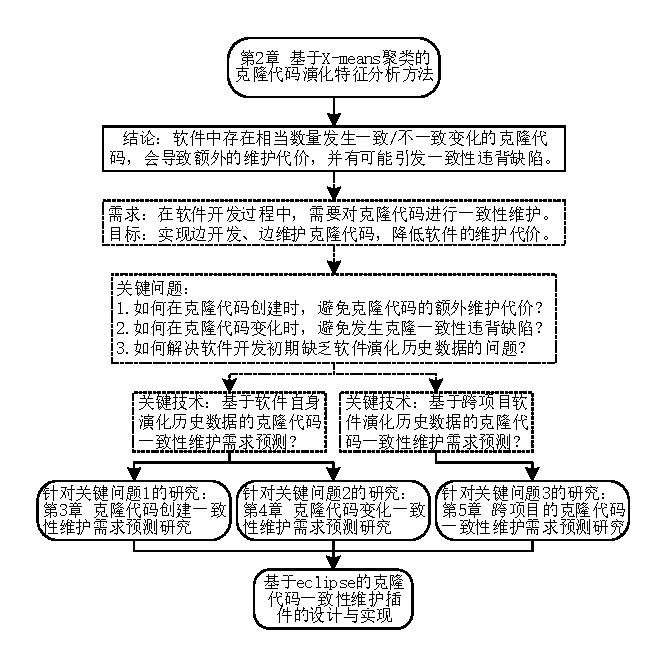
\includegraphics[width = 0.9\textwidth]{framework1.pdf}
\bicaption[framework1]{}{论文主要研究内容及其关系示意图}{Fig.$\!$}
{Main research contents and their relationship in the thesis}
\vspace{-1em}
\end{figure}

本文主要研究四个内容,首先第2章针对演化中的克隆代码难以理解和分析的问题,提出了一种基于X-means聚类的克隆代码演化特征分析方法,通过获取克隆代码演化特征指导克隆代码一致性维护研究。经分析发现:软件中存在相当数量发生变化的克隆代码,其中大部分变化是一致性变化。这不仅会导致额外的维护代价,并有可能引发克隆代码的一致性违背缺陷。因此,在软件开发过程中,需要对克隆代码进行一致性维护,实现边开发、边维护克隆代码,降低软件的维护代价。为了实现上述目标,针对克隆代码的一致性变化会导致额外维护代价和一致性维护缺陷问题,分别在克隆代码创建时(第3章)和克隆代码变化时(第4章)预测克隆代码的一致性维护需求,帮助降低软件维护代价和避免一致性违背缺陷。最后,针对软件开发初期软件缺乏自身历史数据的问题,第5章研究跨项目的克隆代码一致性维护需求预测问题。结合软件开过程,基于eclipse实现了一个克隆代码一致性维护需求预测插件,可以帮助软件开发人员同步的开发和维护克隆代码。

%结论:软件中存在相当数量发生一致/不一致变化的克隆代码,会导致额外的维护代价,并有可能引发一致性违背缺陷。

%%关键问题:1.如何在克隆代码产生时,避免克隆代码的额外维护代价?2.如何在克隆代码变化时,避免发生克隆一致性违背缺陷?3.如何解决软件开发初期缺乏软件演化历史数据的问题?

%关键技术:基于软件自身演化历史数据的克隆代码一致性维护需求预测?
%关键技术:基于跨项目软件演化历史数据的克隆代码一致性维护需求预测?

各章节研究内容安排如下:

第2章研究基于X-means聚类的克隆代码演化特征分析方法,为分析克隆代码演化规律提供了有效的手段,验证了克隆代码一致性需求预测的必要性。首先,使用克隆检测工具检测系统中的克隆代码,并构建系统所有克隆代码的克隆家系,用于描述克隆代码的演化过程。然后,从克隆片段、克隆组和克隆家系三个不同角度提取相应的度量值描述克隆代码及其演化过程。最后,使用聚类分析方法聚类克隆代码、挖掘克隆代码演化特征,帮助开发人员理解克隆代码及其演化过程。

第3章研究克隆代码创建一致性维护需求预测方法,从规避克隆代码产生的角度降低克隆代码的维护代价。通过定义克隆代码创建实例及其一致性维护需求,将问题转化为可以使用机器学习方法解决的分类问题。首先,通过检测系统的克隆代码并构建克隆家系,收集系统中的克隆创建实例。然后,提取代码属性表示被复制的克隆代码,提取上下文属性属性表示被粘贴的克隆代码。最后,使用机器学习方法训练模型,预测克隆代码创建一致性维护需求。

第4章研究克隆代码变化一致性维护需求预测方法,实现克隆代码的同步开发与维护。通过定义克隆代码变化实例及其一致性维护需求,将问题转化为可以使用机器学习方法解决的分类问题。首先,通过检测系统的克隆代码并构建系统克隆家系,收集系统中的克隆变化实例。然后,从克隆组的角度提取代码属性、上下文属性和演化属性三组属性值表示克隆变化实例。最后,使用机器学习方法训练模型,预测克隆代码变化一致性维护需求。

第5章研究跨项目克隆代码一致性维护需求预测实证研究,统一了克隆代码创建和变化实例为克隆实例及其相应的克隆代码一致性维护需求。首先,检测不同软件系统的克隆代码并构建克隆家系,收集并表示克隆代码实例。然后,将软件系统划分为训练系统和测试系统,并使用训练系统数据训练机器学习模型,并在测试系统上预测克隆代码的一致性维护需求。最后,将克隆代码一致性维护需求预测与软件开发过程相结合,实现了一个eclipse插件,帮助实现同步开发和维护克隆代码的一致性。
